\setAuthor{Andres Põldaru}
\setRound{lahtine}
\setYear{2014}
\setNumber{G 8}
\setDifficulty{7}
\setTopic{Staatika}

\prob{Jalgrattur}
Jalgrattur sõidab alla ühtlase kallakuga nõlvast. Kui ta vajutab pidureid täpselt nii kõvasti, et tagumine ratas on peaaegu õhku tõusmas, siis tema kiirus mäest alla sõites ei muutu. Jalgratturist ja rattast koosneva süsteemi massikese asub täpselt kahe ratta vahel kaugusel $h$ maapinnast, rataste telgede vahekaugus on $d$. Kui suur on nõlva ja horisontaalsihi vaheline nurk $\alpha$? Kui suur peab olema ratta ja kaldpinna vaheline hõõrdetegur $\mu$, et jalgrattur saaks kirjeldatud moel pidurdada?

\hint
Kuna tagumine ratas on õhku tõusmas, siis sellele jõude ei rakendu. Ainsad jalgrattale mõjuvad jõud on raskusjõud ning jõud esiratta ja maapinna kontaktpunktis. Lisaks on teada, et peab kehtima nii jõudude kui jõumomentide tasakaal iga punkti suhtes.

\solu
Kuna tagumine ratas on õhku tõusmas, siis sellele jõude ei rakendu. Ainsad jalgrattale mõjuvad jõud on raskusjõud ning jõud esiratta ja maapinna kontaktpunktis. Kuna jalgratas liigub ühtlase kiirusega ning ei hakka pöörlema ega ümber kukkuma, peab jalgrattast ja ratturist koosnevale süsteemile mõjuvate jõudude summa ja ka jõumoment iga punkti suhtes olema null. Raskusjõu tugevus ja suund on teada. Teine jõud peab olema sama suur ja vastassuunaline, et raskusjõudu tasakaalustada. Lisaks peavad jõud paiknema ühel sirgel, et jalgratas koos ratturiga ei hakkaks pöörlema. Järelikult peab massikese olema esiratta ja maapinna kontaktpunkti kohal ning hõõrdejõu ja toereaktsiooni summa on vertikaalne. Lihtsast geomeetriast saame $\alpha=\arctan(\frac{d}{2h})$ ja $\mu\ge\frac{d}{2h}$.
\begin{center}
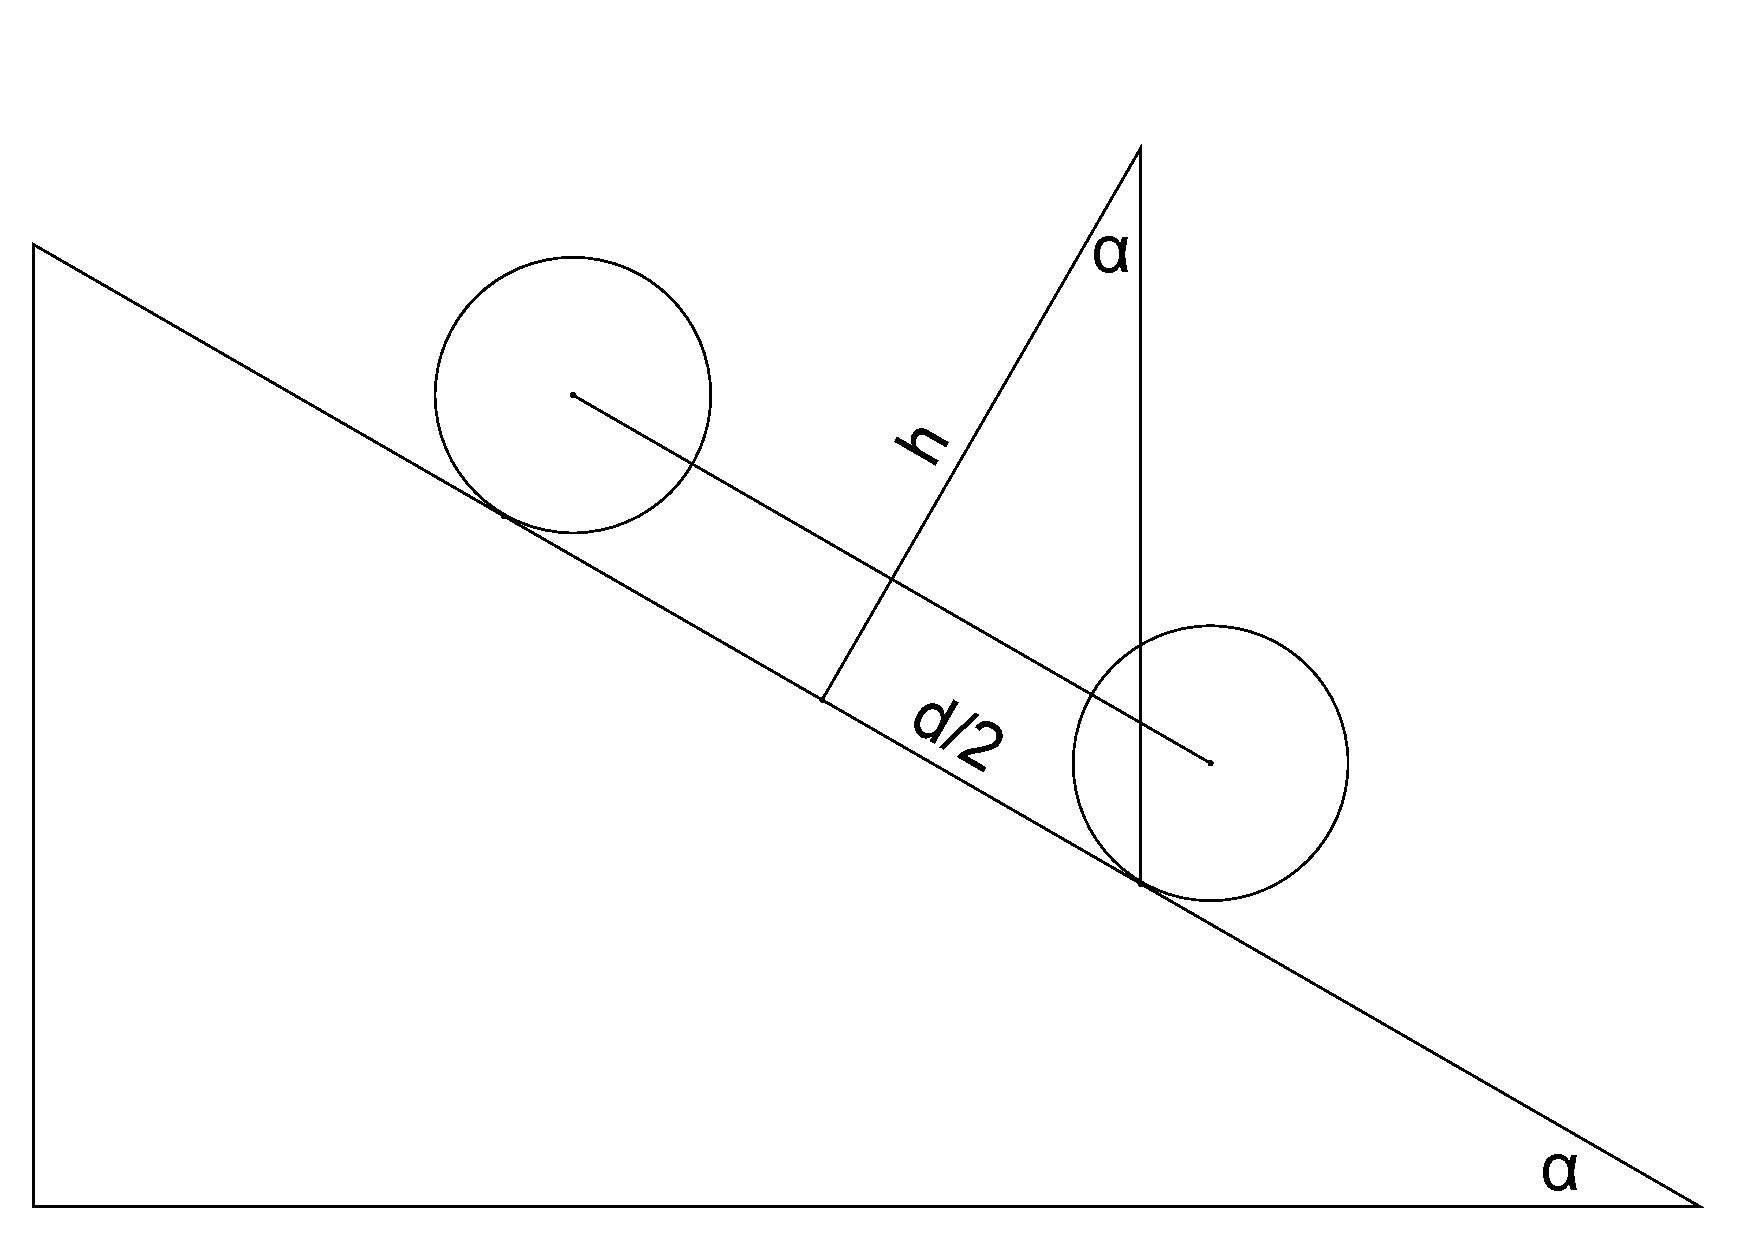
\includegraphics[width=0.6\textwidth]{2014-lahg-08-ratas}
\end{center}

\probeng{Cyclist}
A cyclist is riding down a slope with an even inclination. If he is holding the brakes with exactly such a strength to cause the rear wheel to almost rise into air, then his speed while riding down the slope does not change. The center of mass of the system that consists of the cyclist and the bike is located exactly in the middle of two wheels, at a height $h$ from the ground. The distance between the axes of the wheels is $d$. How big is the angle $\alpha$ between the slope and the horizontal direction? How big has to be the coefficient of friction $\mu$ between the wheel and the ground so that the cyclist could brake like it was described?

\hinteng
Since the rear wheel is on the verge of rising into air there are no forces are applied to it. The only forces applied to the bike are gravity force and the force at the contact point of rear wheel and ground. In addition, it is known that both the force and torque balance has to apply in respect to each point.

\solueng
Because the rear wheel is about to rise into the air then no forces are applied to it. The only forces applied to the bicycle are the gravity force and the force at the contact point of the front wheel and the ground. Because the bicycle is moving with an even velocity and does not start to rotate or fall down the sum of the forces applied to the system consisting of the bicycle and the cyclist has to be zero and the torque with respect to each point has to be zero as well. The value and direction of the gravity force is known. The second force has to be as big and has to have the opposite direction to balance the gravity force. In addition the forces have to be located on the same line so that the bicycle with the cyclist would not start to rotate. Therefore the center of mass has to be above the contact point of the front wheel and the ground and the sum of the friction and normal force is vertical. From simple geometry we get $\alpha=\arctan(\frac{d}{2h})$ and $\mu\ge\frac{d}{2h}$. 
\begin{center}
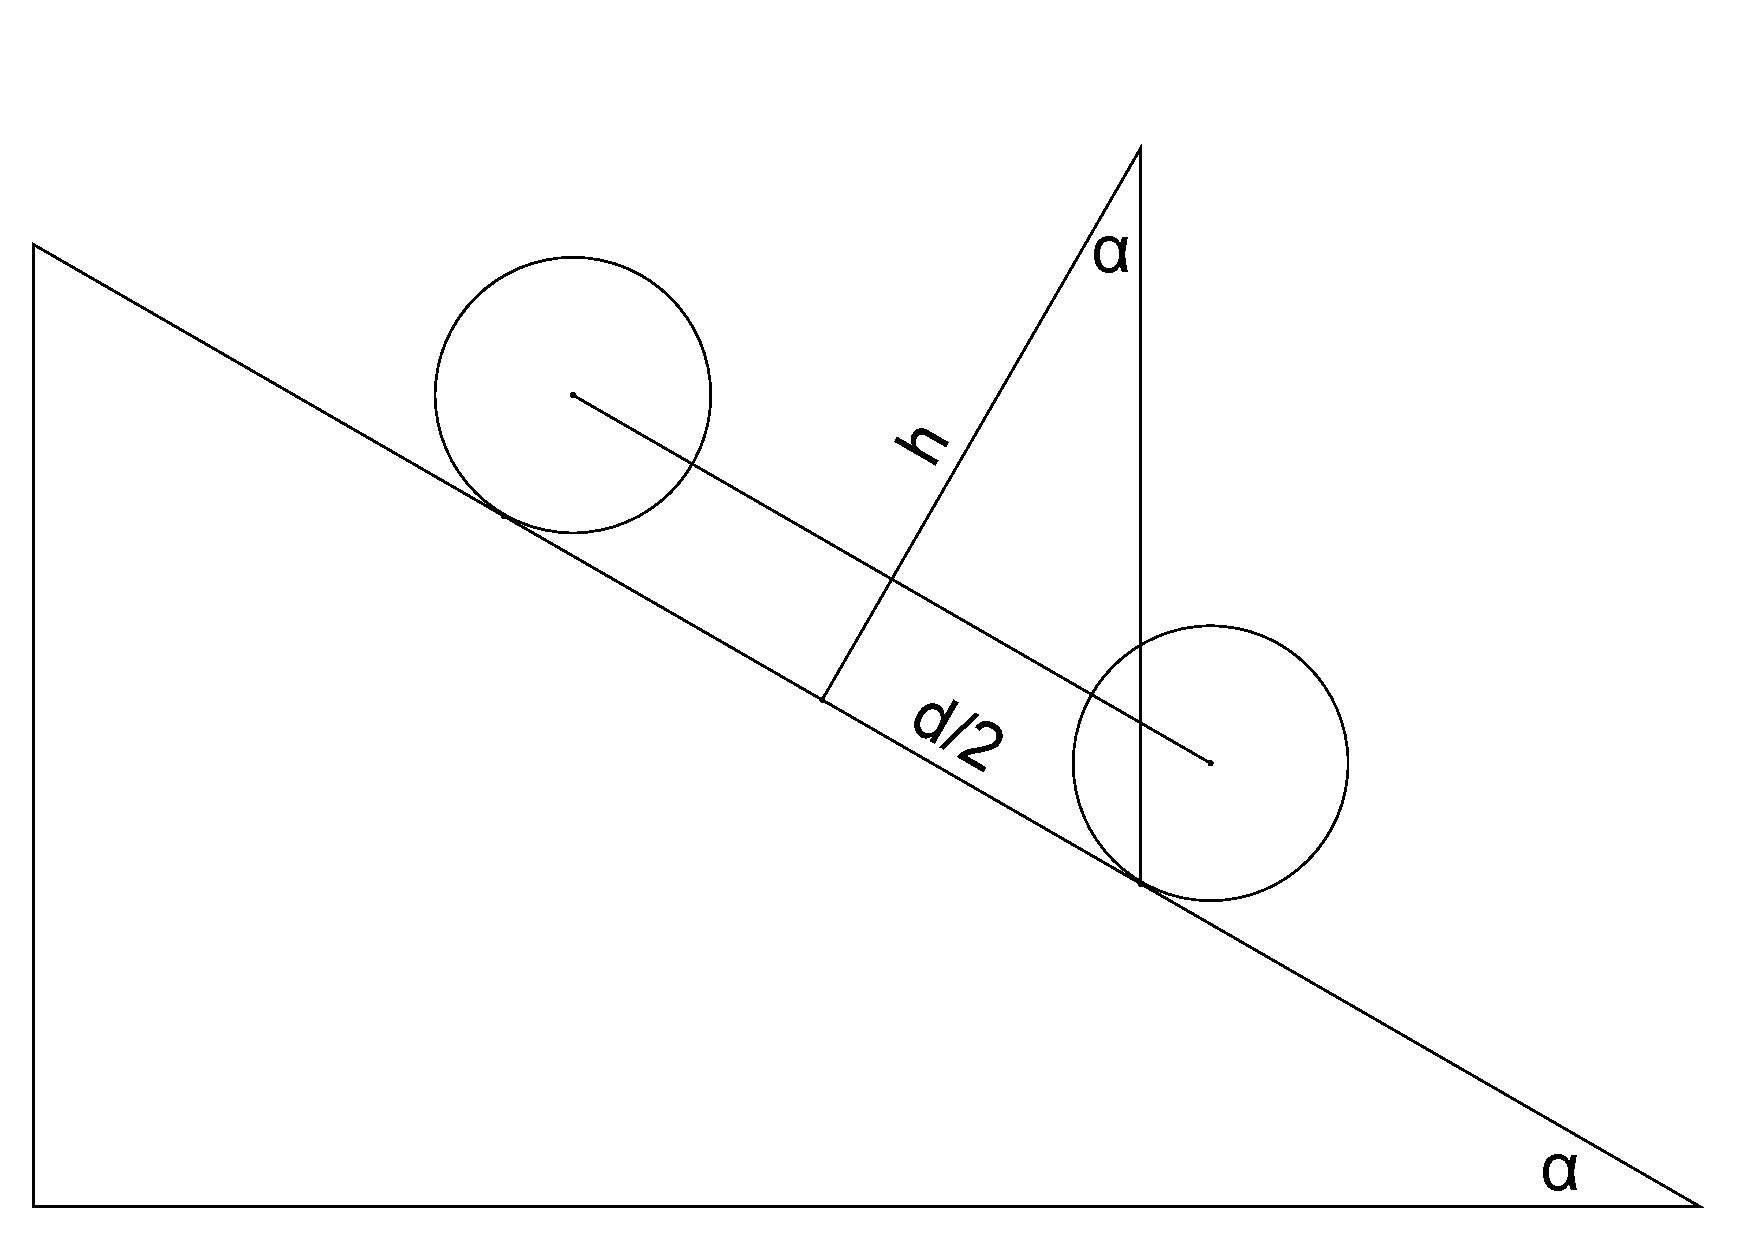
\includegraphics[width=0.6\textwidth]{2014-lahg-08-ratas}
\end{center}
\probend